\documentclass[atiam, article]{rapport} % draft, phelma_black, phelma_normal, kit_de, kit_en, phelma_old
\usepackage{booktabs}


\doctitle{TP Vents}
\title{TP Vents\\Les pertes nuisent-elles\\à la qualité des vents ?}
\titleheader{TP Vents}
\titleone{}
\titletwo{Acoustique}
\titlethree{}
\author{Paul Estève, Étienne André} % Authors for the header
\autpage{ % Authors for the title page
  \begin{tabular}{l}
    Paul Estève \\
    Étienne André
  \end{tabular}
}
\bibliography{biblio}
\supervisor[Encadrants : ]{Jean-Loïc Le Carrou\\Christophe Vergez}
% \supervisorMail{}
\serie{ATIAM 2023/2024}
\date{\today}

\begin{document}

\maketitle


\section{Préparation du TP}


\section{Protocole}

\section{Impédance d'entrée de la flûte}

\subsection{Etude théorique}
\label{subsec:theorie}

On souhaite étudier l'influence des pertes visco-thermiques sur le comportement dynamique de l'instrument. Dans un premier temps, une mesure d'impédance acoustique est réalisée dans différentes configurations, afin d'estimer les fréquences des modes 

Puisqu'on étudie un instrument en première approximation ouvert-ouvert, les fréquences de résonances correspondent aux maxima de l'admittance d'entrée/de sortie et aux minima de l'impédance d'entrée/de sortie.

Notre capteur ayant une surface place plan, on y place l'extrémité "de sortie" de la flûte (opposée à l'embouchure) et on mesure donc l'impédance de sortie de l'instrument.

Le modèle utilisé est celui de Auvray et al. \cite{Auvray2011}. Il permet de modéliser l'impédance de la flûte après le bec, à l'entrée du tuyau, là où le champ acoustique interagit sur le jet.
$$Y_e=Y_c \frac{\cosh \left(\Gamma l+\eta_l\right) \cos \eta_m}{\sinh \left(\Gamma l+\eta_l+\eta_m\right)}$$

avec $Y_c = \frac{S}{\rho c S_m}$, $S_m$ la section de la bouche, $l$ la longueur du tuyau, $\Gamma$ le nombre d'onde complexe et $\eta_i = \arg \tanh\left(\frac{Z_i}{Z_c}\right)$.

En utilisant la méthode de l'impédance ramenée, on peut en déduire une formule théorique de l'impédance de sortie.

Si $$\begin{pmatrix}
    P_s\\U_s
\end{pmatrix} =
M
\begin{pmatrix}
    P_e\\U_e
\end{pmatrix}$$

Avec $M = \begin{pmatrix}A & B\\C&D\end{pmatrix}$, on a $Y_s = \frac{U_s}{P_s} = \frac{C + D Y_e}{A + B Y_e}$. 

Pour un tuyau cylindrique de longueur $l$, la matrice $M$ est définie comme

\begin{equation}
    M = \begin{pmatrix}
        \cosh \Gamma l & Z_c \sinh \Gamma l \\
        Z_c^{-1} \sinh \Gamma l & \cosh \Gamma l
    \end{pmatrix}
    \label{eq:mat_trans_cylindre}
\end{equation}

avec $Z_c = \sqrt{\frac{Z_v}{Y_t}}$ pour tenir compte des pertes visqueuses et thermiques comme indiqué durant le cours\cite{Vergez4}.

\subsection{Mesures}

On effectue à l'aide d'un capteur d'impédance des mesures pour 4 configurations :
\begin{enumerate}
    \item Cylindre seul
    \item Cylindre avec bec
    \item Cylindre avec stack inséré
    \item Cylindre avec bec et stack
\end{enumerate}

La position du stack changeant grandement son influence sur le comportement de l'instrument, on effectue les mesures dans l'ordre des configurations indiqués avant de passer à la partie dynamique avec bouche artificielle. De cette manière, toutes les mesures avec stack analysées dans cette partie et la suivante 

Etant donné que l'on étudie les premiers registres on  mesure l'impédance de $\SI{100}{\Hz}$ jusqu'à $\SI{4}{\kHz}$. 
Le temps de sweep est de $\SI{2}{\s}$, avec un moyennage sur 10 mesures.
Mesurer une plus grande plage était possible, mais on souhaite maximiser le nombre de points et de temps de mesure dans la région d'intérêt.

% Pour vérifier la cohérence de l'ensemble des mesures, on analyse d'abord

\subsubsection{Impédance du cylindre seul et vérification de la cohérence des mesures}

On vérifie dans un premier temps que les mesures d'impédances sont cohérentes en comparant l'impédance d'entrée\footnote{Un cylindre étant symétrique, on parle ici successivement d'impédance d'entrée et d'impédance de sortie : elles sont égales.} mesurée pour le cylindre, avec les formules théoriques du cours \cite{Vergez4}. On utilise les formules avec l'approximation des tuyaux larges (nombre de Stokes $r_v$ grand permet un développement à l'ordre 1 de $\Gamma$) et une prise en compte de l'impédance de rayonnement pour un instrument non bafflé.

\begin{itemize}
    \item \textbf{Valeur des paramètres :}
    \begin{align*}
        \begin{array}{lll}
            l & = \SI{183e-3}{\meter} & \text{(Longueur du cylindre)} \\
            D & = \SI{19e-3}{\meter} & \text{(Diamètre du cylindre)} \\
            R & = \frac{D}{2} & \text{(Rayon du cylindre)} \\
            T & = \SI{21.7}{\celsius} & \text{(Température de la salle)}\\
            \rho_0 & = 1.292 \left(\frac{273.15}{T}\right) & \text{(Masse volumique de l'air, \si{\kg.\m^{-3}})} \\
            S & = \pi R^2 & \text{(Section transversale du cylindre)} \\
            c & = 20.05 \sqrt{T} & \text{(Vitesse du son dans l'air)}
        \end{array}
    \end{align*}

    \item \textbf{Calcul de l'impédance de rayonnement (\(Z_r\)) :}
    \begin{align*}
        \begin{array}{lll}
            \alpha_1 & = 1.044 \\
            \mu & \simeq 8.9 \times 10^{-15} T^3 - 3.2 \times 10^{-11} T^2 + 6.3 \times 10^{-8} T + 2.4 \times 10^{-6} & \text{(Viscosité de l'air)}\\
        \end{array}
    \end{align*}
    \begin{align*}
        \begin{array}{lll}
            l_v & = \frac{\mu}{\rho_0 c} & \text{(Epaisseur de la couche visqueuse)} \\
            k_v & = \sqrt{-j \frac{2\pi f}{c l_v}} & \text{(Nombre d'onde de diffusion visqueuse)} \\
            r_v & = \lvert k_v R \rvert & \text{(Nombre de Stokes)} \\
            v_\phi & = c \left(1 - \frac{\alpha_1}{r_v}\right) & \text{(Vitesse de phase de l'onde acoustique)} \\
            k & = \frac{2\pi f}{v_\phi} & \text{(Nombre d'onde)} \\
            \Delta l & = 0.61 R & \text{(Correction de longueur due au rayonnement)} \\
            Z_r & = Z_c \left(jk\Delta l + \frac{1}{4}(kR)^2\right) & \text{(Impédance de rayonnement)}
        \end{array}
    \end{align*}

    \item \textbf{Calcul de l'impédance d'entrée (\(Z_e\)) dans le cadre des guides cylindriques "larges" :}
    \begin{align*}
        \begin{array}{lll}
            \Gamma & = j2\pi\frac{f}{c} + (1 + j)3 \times 10^{-5} \sqrt{f} \frac{1}{R} & \text{(Paramètre complexe pour les pertes viscothermiques)} \\
            Z_e & = \lvert Z_c \tanh(\Gamma l + \text{arctanh}(Z_r/Z_c)) \rvert & \text{(Impédance d'entrée)}
        \end{array}
        \label{eq:ze-cyl}
    \end{align*}
\end{itemize}

Les paramètres et formules citées permettent de tracer l'impédance d'entrée théorique. On compare dans la figure \ref{fig:ze-cyl} cette impédance théorique et l'impédance d'entrée mesurée. Les courbes se superposent quasi parfaitement à partir de $\SI{360}{\Hz}$. Le modèle est bien en adéquation avec la mesure. On conclue pour la suite que nos mesures d'impédance sont cohérentes.

\begin{figure}
    \centering
    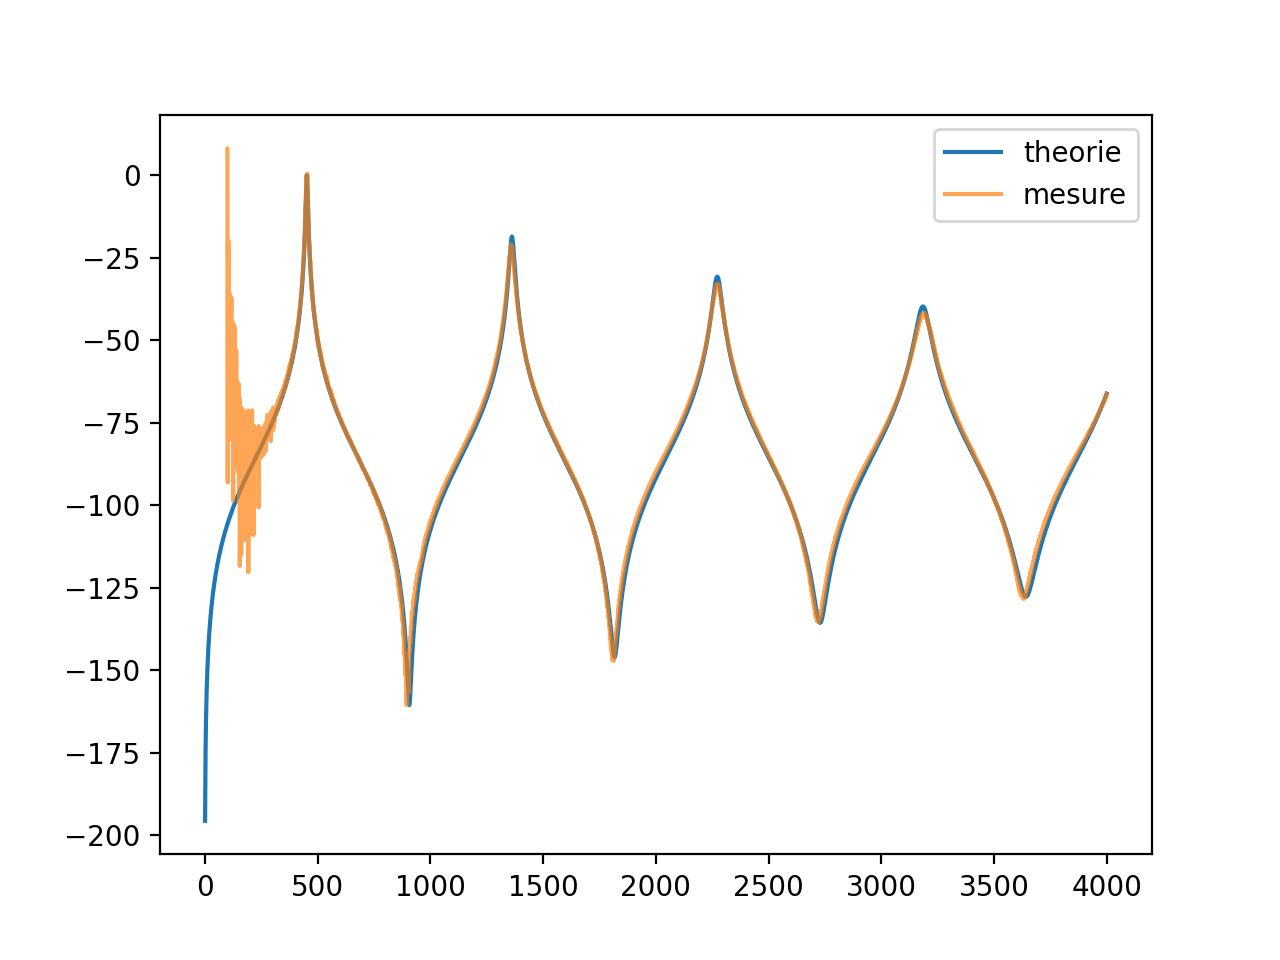
\includegraphics[width=.5\textwidth]{vents/images_vents/impedance_cylindre.png}
    \caption{Impédance du cylindre}
    \label{fig:ze-cyl}
\end{figure}

\subsubsection{Admittance des différentes configurations}

Ne connaissant pas tous les paramètres du modèle plus complexe expliqué dans la section \ref{subsec:theorie}, en particulier les $\eta_i$, on modélise l'admittance de sortie par une somme de passe-bande du second ordre :

$$
Y_s=\sum_{n=1}^{\infty} \frac{j \omega Y_n}{\omega_n^2-\omega^2+j Q_n^{-1} \omega_n \omega}
$$

Cette modélisation, si elle s'avère cohérente avec nos mesures, permet d'estimer les facteurs de qualité des différents modes, liés aux amortissements.

\begin{table}[H]
    \centering
    \begin{tabular}{ccc}
\toprule
$f_n$ & $Q_n$ & $Y_n$ \\ \midrule
180 & 8 & 1032.07 \\
898 & 75 & 3096.22 \\
1810 & 70 & 3440.25 \\
2720 & 50 & 4128.30 \\
3630 & 50 & 4128.30 \\
\bottomrule\\
    \end{tabular}
    \caption{Paramètres du modèle pour le cylindre seul}
    \label{tab:param_cylindre}
\end{table}

\begin{table}[H]
    \centering
    \begin{tabular}{ccc}
\toprule
$f_n$ & $Q_n$ & $Y_n$ \\ \midrule
190 & 5 & 1032.07 \\
877 & 13 & 2545.78 \\
1770 & 12 & 3096.22 \\
2710 & 17 & 4472.32 \\
3555 & 20 & 2752.20 \\
\bottomrule\\
    \end{tabular}
    \caption{Paramètres du modèle pour le cylindre avec stack}
    \label{tab:param_cylindre+stack}
\end{table}

\begin{table}[H]
    \centering
    \begin{tabular}{ccc}
\toprule
$f_n$ & $Q_n$ & $Y_n$ \\ \midrule
508 & 16 & 2201.76 \\
1045 & 57 & 2064.15 \\
1592 & 65 & 2064.15 \\
2160 & 38 & 2752.20 \\
2708 & 60 & 2752.20 \\
3308 & 45 & 3440.25 \\
3879 & 50 & 4128.30 \\
\bottomrule\\
    \end{tabular}
    \caption{Paramètres du modèle pour le cylindre et le bec}
    \label{tab:param_cylindre+bec}
\end{table}

\begin{table}[H]
    \centering
    \begin{tabular}{ccc}
\toprule
$f_n$ & $Q_n$ & $Y_n$ \\ \midrule
498 & 7 & 2201.76 \\
1045 & 20 & 1857.73 \\
1575 & 20 & 1720.12 \\
2161 & 20 & 2752.20 \\
2702 & 30 & 2408.17 \\
3265 & 20 & 3440.25 \\
3845 & 40 & 1376.10 \\
\bottomrule\\
    \end{tabular}
    \caption{Paramètres du modèle pour le cylindre avec stack et le bec}
    \label{tab:param_cylindre+stack+bec}
\end{table}



\section{Comportement dynamique de la flûte}

Dans cette seconde partie du TP, une bouche artificielle permet de contrôler la pression d'entrée dans le bec. En faisant varier la pression, on s'attend à entendre l'apparition d'un premier régime (bifurcation de Hopf), puis à des bifurcations à chacuns des régimes correspondant aux fréquences des maxima de l'admittance de sortie mesurées dans la section précédente.

\subsection{Protocole}

Pour chaque configuration, on mesure % TODO insert description de la mesure

\printbibliography

\end{document}
